% Options for packages loaded elsewhere
\PassOptionsToPackage{unicode}{hyperref}
\PassOptionsToPackage{hyphens}{url}
%
\documentclass[
  english,
  man]{apa6}
\usepackage{lmodern}
\usepackage{amsmath}
\usepackage{ifxetex,ifluatex}
\ifnum 0\ifxetex 1\fi\ifluatex 1\fi=0 % if pdftex
  \usepackage[T1]{fontenc}
  \usepackage[utf8]{inputenc}
  \usepackage{textcomp} % provide euro and other symbols
  \usepackage{amssymb}
\else % if luatex or xetex
  \usepackage{unicode-math}
  \defaultfontfeatures{Scale=MatchLowercase}
  \defaultfontfeatures[\rmfamily]{Ligatures=TeX,Scale=1}
\fi
% Use upquote if available, for straight quotes in verbatim environments
\IfFileExists{upquote.sty}{\usepackage{upquote}}{}
\IfFileExists{microtype.sty}{% use microtype if available
  \usepackage[]{microtype}
  \UseMicrotypeSet[protrusion]{basicmath} % disable protrusion for tt fonts
}{}
\makeatletter
\@ifundefined{KOMAClassName}{% if non-KOMA class
  \IfFileExists{parskip.sty}{%
    \usepackage{parskip}
  }{% else
    \setlength{\parindent}{0pt}
    \setlength{\parskip}{6pt plus 2pt minus 1pt}}
}{% if KOMA class
  \KOMAoptions{parskip=half}}
\makeatother
\usepackage{xcolor}
\IfFileExists{xurl.sty}{\usepackage{xurl}}{} % add URL line breaks if available
\IfFileExists{bookmark.sty}{\usepackage{bookmark}}{\usepackage{hyperref}}
\hypersetup{
  pdftitle={Are we all on the same page? Subfield differences in open science practice},
  pdfauthor={Christina Riochios1 \& Jenny L. Richmond1},
  pdflang={en-EN},
  pdfkeywords={keywords},
  hidelinks,
  pdfcreator={LaTeX via pandoc}}
\urlstyle{same} % disable monospaced font for URLs
\usepackage{graphicx}
\makeatletter
\def\maxwidth{\ifdim\Gin@nat@width>\linewidth\linewidth\else\Gin@nat@width\fi}
\def\maxheight{\ifdim\Gin@nat@height>\textheight\textheight\else\Gin@nat@height\fi}
\makeatother
% Scale images if necessary, so that they will not overflow the page
% margins by default, and it is still possible to overwrite the defaults
% using explicit options in \includegraphics[width, height, ...]{}
\setkeys{Gin}{width=\maxwidth,height=\maxheight,keepaspectratio}
% Set default figure placement to htbp
\makeatletter
\def\fps@figure{htbp}
\makeatother
\setlength{\emergencystretch}{3em} % prevent overfull lines
\providecommand{\tightlist}{%
  \setlength{\itemsep}{0pt}\setlength{\parskip}{0pt}}
\setcounter{secnumdepth}{-\maxdimen} % remove section numbering
% Make \paragraph and \subparagraph free-standing
\ifx\paragraph\undefined\else
  \let\oldparagraph\paragraph
  \renewcommand{\paragraph}[1]{\oldparagraph{#1}\mbox{}}
\fi
\ifx\subparagraph\undefined\else
  \let\oldsubparagraph\subparagraph
  \renewcommand{\subparagraph}[1]{\oldsubparagraph{#1}\mbox{}}
\fi
% Manuscript styling
\usepackage{upgreek}
\captionsetup{font=singlespacing,justification=justified}

% Table formatting
\usepackage{longtable}
\usepackage{lscape}
% \usepackage[counterclockwise]{rotating}   % Landscape page setup for large tables
\usepackage{multirow}		% Table styling
\usepackage{tabularx}		% Control Column width
\usepackage[flushleft]{threeparttable}	% Allows for three part tables with a specified notes section
\usepackage{threeparttablex}            % Lets threeparttable work with longtable

% Create new environments so endfloat can handle them
% \newenvironment{ltable}
%   {\begin{landscape}\centering\begin{threeparttable}}
%   {\end{threeparttable}\end{landscape}}
\newenvironment{lltable}{\begin{landscape}\centering\begin{ThreePartTable}}{\end{ThreePartTable}\end{landscape}}

% Enables adjusting longtable caption width to table width
% Solution found at http://golatex.de/longtable-mit-caption-so-breit-wie-die-tabelle-t15767.html
\makeatletter
\newcommand\LastLTentrywidth{1em}
\newlength\longtablewidth
\setlength{\longtablewidth}{1in}
\newcommand{\getlongtablewidth}{\begingroup \ifcsname LT@\roman{LT@tables}\endcsname \global\longtablewidth=0pt \renewcommand{\LT@entry}[2]{\global\advance\longtablewidth by ##2\relax\gdef\LastLTentrywidth{##2}}\@nameuse{LT@\roman{LT@tables}} \fi \endgroup}

% \setlength{\parindent}{0.5in}
% \setlength{\parskip}{0pt plus 0pt minus 0pt}

% \usepackage{etoolbox}
\makeatletter
\patchcmd{\HyOrg@maketitle}
  {\section{\normalfont\normalsize\abstractname}}
  {\section*{\normalfont\normalsize\abstractname}}
  {}{\typeout{Failed to patch abstract.}}
\patchcmd{\HyOrg@maketitle}
  {\section{\protect\normalfont{\@title}}}
  {\section*{\protect\normalfont{\@title}}}
  {}{\typeout{Failed to patch title.}}
\makeatother
\shorttitle{Subfield }
\keywords{keywords\newline\indent Word count: X}
\DeclareDelayedFloatFlavor{ThreePartTable}{table}
\DeclareDelayedFloatFlavor{lltable}{table}
\DeclareDelayedFloatFlavor*{longtable}{table}
\makeatletter
\renewcommand{\efloat@iwrite}[1]{\immediate\expandafter\protected@write\csname efloat@post#1\endcsname{}}
\makeatother
\usepackage{lineno}

\linenumbers
\usepackage{csquotes}
\ifxetex
  % Load polyglossia as late as possible: uses bidi with RTL langages (e.g. Hebrew, Arabic)
  \usepackage{polyglossia}
  \setmainlanguage[]{english}
\else
  \usepackage[shorthands=off,main=english]{babel}
\fi
\ifluatex
  \usepackage{selnolig}  % disable illegal ligatures
\fi
\newlength{\cslhangindent}
\setlength{\cslhangindent}{1.5em}
\newlength{\csllabelwidth}
\setlength{\csllabelwidth}{3em}
\newenvironment{CSLReferences}[2] % #1 hanging-ident, #2 entry spacing
 {% don't indent paragraphs
  \setlength{\parindent}{0pt}
  % turn on hanging indent if param 1 is 1
  \ifodd #1 \everypar{\setlength{\hangindent}{\cslhangindent}}\ignorespaces\fi
  % set entry spacing
  \ifnum #2 > 0
  \setlength{\parskip}{#2\baselineskip}
  \fi
 }%
 {}
\usepackage{calc}
\newcommand{\CSLBlock}[1]{#1\hfill\break}
\newcommand{\CSLLeftMargin}[1]{\parbox[t]{\csllabelwidth}{#1}}
\newcommand{\CSLRightInline}[1]{\parbox[t]{\linewidth - \csllabelwidth}{#1}\break}
\newcommand{\CSLIndent}[1]{\hspace{\cslhangindent}#1}

\title{Are we all on the same page? Subfield differences in open science practice}
\author{Christina Riochios\textsuperscript{1} \& Jenny L. Richmond\textsuperscript{1}}
\date{}


\authornote{

School of Psychology, UNSW

The authors made the following contributions. Christina Riochios: Conceptualization, Methodology, Investigation, Data curation, Visualisation, Formal Analysis, Writing - Original Draft Preparation, Writing - Review \& Editing; Jenny L. Richmond: Conceptualization, Methodology, Formal Analysis, Writing - Original Draft Preparation, Writing - Review \& Editing, Supervision.

}

\affiliation{\vspace{0.5cm}\textsuperscript{1} University of New South Wales}

\abstract{
One or two sentences providing a \textbf{basic introduction} to the field, comprehensible to a scientist in any discipline.

Two to three sentences of \textbf{more detailed background}, comprehensible to scientists in related disciplines.

One sentence clearly stating the \textbf{general problem} being addressed by this particular study.

One sentence summarizing the main result (with the words ``\textbf{here we show}'' or their equivalent).

Two or three sentences explaining what the \textbf{main result} reveals in direct comparison to what was thought to be the case previously, or how the main result adds to previous knowledge.

One or two sentences to put the results into a more \textbf{general context}.

Two or three sentences to provide a \textbf{broader perspective}, readily comprehensible to a scientist in any discipline.
}



\begin{document}
\maketitle

The field of psychology, like many other scientific disciplines, is currently facing a replication crisis, in which researchers are struggling to replicate existing findings. In 2015, a group of 270 psychological researchers attempted to replicate the findings of 100 psychology experiments. Whilst 97\% of the original studies generated statistically significant findings, only 36\% of the replication attempts were statistically significant. In addition, the replicated effects were, on average, 50\% smaller than the original effects (Collaboration, 2015). These findings illustrate the lack of replicability in psychological research and the pressing need to rectify flawed research practices.

One strategy that has been used to combat psychology's replication crisis is open science. Open science practices are those that increase the transparency of, and access to, scientific research (Klein et al., 2018). Open data and open material practices, for example, involve researchers sharing their materials and raw data on publicly accessible online repositories. These practices make it easier for others to replicate a study's methods and reproduce its results (Klein et al., 2018).

(Hardwicke et al., 2018).

To encourage researchers to employ open science practices, many psychology journals have started awarding Open Science Badges. In 2013, the Center for Open Science established three Open Science Badges: Open Data, Open Materials and Preregistered, to acknowledge and reward articles for their use of open science practices (Center for Open Science, 2021). The Open Data Badge and the Open Materials Badge are awarded when the data and materials that are required to reproduce the methods and results of a study are shared publicly online, whilst the Preregistered Badge is awarded when the study's design and hypotheses are publicly archived prior to data collection. To date, 75 journals have adopted the COS's Open Science badges, close to 40 being psychology journals (Center for Open Science, 2021).

At Psychological Science, the Association of Psychological Science's flagship journal, Open Science Badges appear to have successfully encouraged authors to adopt open science practices. In 2016, Kidwell et al.~measured rates of data and material sharing in the 18 months before and after Open Science Badges were implemented at Psychological Science, on the 1st of January 2014 (Kidwell et al., 2016). Kidwell et al.~found that authors' use of data sharing practices increased dramatically from 2.5\%, prior to badges, to 39.4\%, following badges. The use of material sharing practices also rose from 12.7\% to 30.3\%. Data and material sharing in control journals, such as the Journal of Personality and Social Psychology, which did not award badges, remained low over the same time period (Kidwell et al., 2016). These results led Kidwell et al.~to conclude that Open Science Badges successfully incentivise the uptake of open science practices.

Whilst the support for open science continues to grow, it is not yet clear whether researchers' use of open science practices is consistent across different fields within psychology. Notably, developmental psychology has received significant criticism for its lack of receptivity towards open science. As Figure 1 illustrates, prominent developmental researchers, Prof Michael Frank and Dr.~Jennifer Pfeifer, have labelled the Society for Research in Child Development's (SRCD) open science policy as `weak' and as one that `undervalues openness.' More recently, the Editor-in-Chief of Infant and Child Development, Prof Moin Syed, stated that the uptake of open science within the field of developmental psychology has been `slow and uneven' (Syed, 2020). A survey supporting these viewpoints showed that, on average, 80\% of Child Development authors felt their institutions failed to provide adequate guidance or financial support for sharing data, (SRCD Task Force on Scientific Integrity and Openness Survey (2017), cited in Gennetian et al., (Gennetian, Tamis-LeMonda, \& Frank, 2020). Overall, this evidence indicates that developmental researchers may be slower to adopt open science practices than those in other psychological disciplines.

FIGURE 1

Meta-research, the study of research itself, can empirically assess whether developmental psychology is truly behind in the open science movement. Previous investigations, including Kidwell et al. (Kidwell et al., 2016), have revealed that open science incentives can increase the use of open science practices. However, what remains unclear is whether the uptake of open science has been consistent across psychological subfields. To address this research question, Study 1A utilised open data from the Kidwell et al.~study to examine whether rates of data and material sharing, following the implementation of Open Science Badges at Psychological Science, differed as a function of subfield. Whilst we expected to observe subfield differences in the use of open science practices, the nature and magnitude of these differences remained unclear. Study 1A was preregistered at the Open Science Framework: \url{https://osf.io/3tsmy/}.

\hypertarget{methods}{%
\section{Methods}\label{methods}}

We report how we determined our sample size, all data exclusions (if any), all manipulations, and all measures in the study.

\hypertarget{participants}{%
\subsection{Participants}\label{participants}}

\hypertarget{material}{%
\subsection{Material}\label{material}}

\hypertarget{procedure}{%
\subsection{Procedure}\label{procedure}}

\hypertarget{data-analysis}{%
\subsection{Data analysis}\label{data-analysis}}

We used R {[}Version 4.0.3; R Core Team (2020){]} and the R-packages \emph{afex} {[}Version 1.0.1; Singmann, Bolker, Westfall, Aust, and Ben-Shachar (2021){]}, \emph{apa} {[}Version 0.3.3; Gromer (2020); Aust and Barth (2020){]}, \emph{dplyr} {[}Version 1.0.7; Wickham, François, Henry, and Müller (2021){]}, \emph{forcats} {[}Version 0.5.1; Wickham (2021a){]}, \emph{ggeasy} {[}Version 0.1.3; Carroll, Schep, and Sidi (2021){]}, \emph{gghalves} {[}Version 0.1.1; Tiedemann (2020){]}, \emph{ggplot2} {[}Version 3.3.5; Wickham (2016){]}, \emph{ggsignif} {[}Version 0.6.3; Constantin and Patil (2021){]}, \emph{goodshirt} {[}Version 0.2.2; Gruer (2021){]}, \emph{here} {[}Version 1.0.1; Müller (2020){]}, \emph{janitor} {[}Version 2.1.0; Firke (2021){]}, \emph{lme4} {[}Version 1.1.27.1; Bates, Mächler, Bolker, and Walker (2015){]}, \emph{Matrix} {[}Version 1.3.4; Bates and Maechler (2021){]}, \emph{papaja} {[}Version 0.1.0.9997; Aust and Barth (2020){]}, \emph{patchwork} {[}Version 1.1.1; Pedersen (2020){]}, \emph{purrr} {[}Version 0.3.4; Henry and Wickham (2020){]}, \emph{readr} {[}Version 2.0.1; Wickham and Hester (2021){]}, \emph{report} {[}Version 0.3.5; Makowski, Ben-Shachar, Patil, and Lüdecke (2021){]}, \emph{stringr} {[}Version 1.4.0; Wickham (2019){]}, \emph{tibble} {[}Version 3.1.4; Müller and Wickham (2021){]}, \emph{tidyr} {[}Version 1.1.3; Wickham (2021b){]}, and \emph{tidyverse} {[}Version 1.3.1; Wickham et al. (2019){]} for all our analyses.

\hypertarget{a-results}{%
\section{1A Results}\label{a-results}}

\hypertarget{adata-scores-text}{%
\section{1AData scores text}\label{adata-scores-text}}

As illustrated in Figure 1, the two-way between-subjects ANOVA generated a significant main effect of time period, \(F(2, 310) = 11.29\), \(\mathit{MSE} = 41.51\), \(p < .001\), \(\hat{\eta}^2_G = .068\). However, the main effect of subfield, \(F(3, 310) = 2.23\), \(\mathit{MSE} = 41.51\), \(p = .085\), \(\hat{\eta}^2_G = .021\), and the interaction between time period and subfield, \(F(6, 310) = 1.57\), \(\mathit{MSE} = 41.51\), \(p = .157\), \(\hat{\eta}^2_G = .029\), were not statistically significant. Articles published in the latter part of 2014 had significantly higher open data scores than article published in the first half of the year, \(t(99.74) = -2.87\), \(p = .005\), however there was no further increase across the early part of 2015,\(t(132.74) = -0.86\), \(p = .391\). Critically, there was no significant difference in the open data scores as a function of subfield (see Figure 1a).

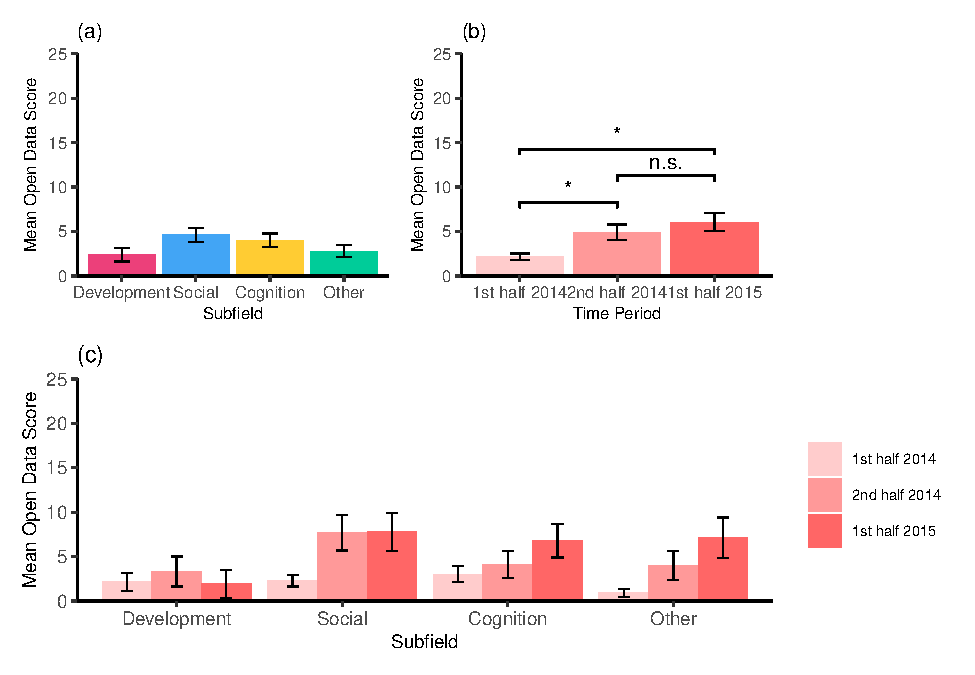
\includegraphics{icd_special_issue_files/figure-latex/1A-d-plots-1.pdf}

\emph{Figure 1}: Mean open data scores for article published in 2014 and 2015, as a function of subfield and time period.

\begin{table}[tbp]

\begin{center}
\begin{threeparttable}

\caption{\label{tab:1A-m-anova}Between-subjects ANOVA for Open Materials Scores}

\begin{tabular}{lllllll}
\toprule
Effect & \multicolumn{1}{c}{$F$} & \multicolumn{1}{c}{$\mathit{df}_1$} & \multicolumn{1}{c}{$\mathit{df}_2$} & \multicolumn{1}{c}{$\mathit{MSE}$} & \multicolumn{1}{c}{$p$} & \multicolumn{1}{c}{$\hat{\eta}^2_G$}\\
\midrule
Time period & 4.74 & 2 & 310 & 32.16 & .009 & .030\\
Subfield groups & 4.03 & 3 & 310 & 32.16 & .008 & .038\\
Time period $\times$ Subfield groups & 0.85 & 6 & 310 & 32.16 & .530 & .016\\
\bottomrule
\end{tabular}

\end{threeparttable}
\end{center}

\end{table}

\hypertarget{amaterial-scores-text}{%
\section{1AMaterial scores text}\label{amaterial-scores-text}}

In contrast, for open materials scores, two-way between-subjects ANOVA generated a significant main effect of subfield, \(F(3, 310) = 4.03\), \(\mathit{MSE} = 32.16\), \(p = .008\), \(\hat{\eta}^2_G = .038\), and a significant main effect of time period, \(F(2, 310) = 4.74\), \(\mathit{MSE} = 32.16\), \(p = .009\), \(\hat{\eta}^2_G = .030\). However the interaction between time period and subfield, \(F(6, 310) = 0.85\), \(\mathit{MSE} = 32.16\), \(p = .530\), \(\hat{\eta}^2_G = .016\), was not statistically significant. Papers in developmental psychology had lower open materials scores than those in both social, \(t(153.62) = -2.75\), \(p = .007\), and cognition, \(t(153.74) = -3.20\), \(p = .002\), but developmental open materials scores did not differ from papers allocated to the other subfield category, \(t(137.95) = -1.19\), \(p = .236\). Open materials scores increased incrementally across 2014 and 2015; papers published in the first half of 2015 had significantly higher open materials scores than those published in the first half of 2014,\(t(95.44) = -2.55\), \(p = .012\).

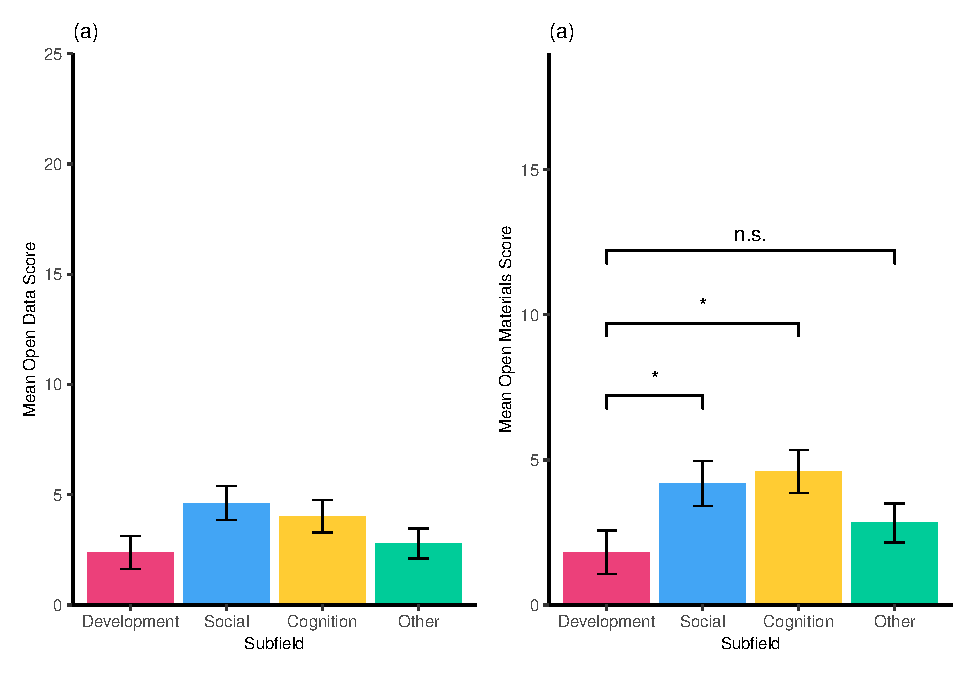
\includegraphics{icd_special_issue_files/figure-latex/1A-m-plots-1.pdf}

\textbf{Figure 2}: Mean open materials scores for articles published in 2014 and 2015, as a function of subfield and time period.

\hypertarget{b-results}{%
\section{1B Results}\label{b-results}}

\hypertarget{bdata-scores-text}{%
\subsection{1BData scores text}\label{bdata-scores-text}}

Consistent with the results from Study 1A, open data scores also increased significantly across 2019 and 2020, \(F(2, 181) = 3.68\), \(\mathit{MSE} = 70.92\), \(p = .027\), \(\hat{\eta}^2_G = .039\), however across this time period, open data scores differed significantly by subfield, \(F(3, 181) = 3.31\), \(\mathit{MSE} = 70.92\), \(p = .021\), \(\hat{\eta}^2_G = .052\). The interaction between time period and subfield, \(F(6, 181) = 1.11\), \(\mathit{MSE} = 70.92\), \(p = .358\), \(\hat{\eta}^2_G = .035\), was not statistically significant. When we compared the open data scores from papers published in developmental psychology to each of the other subfield categories (Figure 2a), we found that papers in developmental psychology had significantly lower open data scores than papers in cognition, \(t(58.75) = -2.65\), \(p = .010\). The magnitude of open data scores did not differ from papers published in social psychology, \(t(71.68) = -0.42\), \(p = .675\) or those that fell into the other category, \(t(71.12) = -0.31\), \(p = .756\). In terms of changes over time, open data scores increased significantly from late 2019 into 2020, \(t(126.73) = -2.70\), \(p = .008\), but were stable across 2020, \(t(62.65) = 0.98\), \(p = .331\).

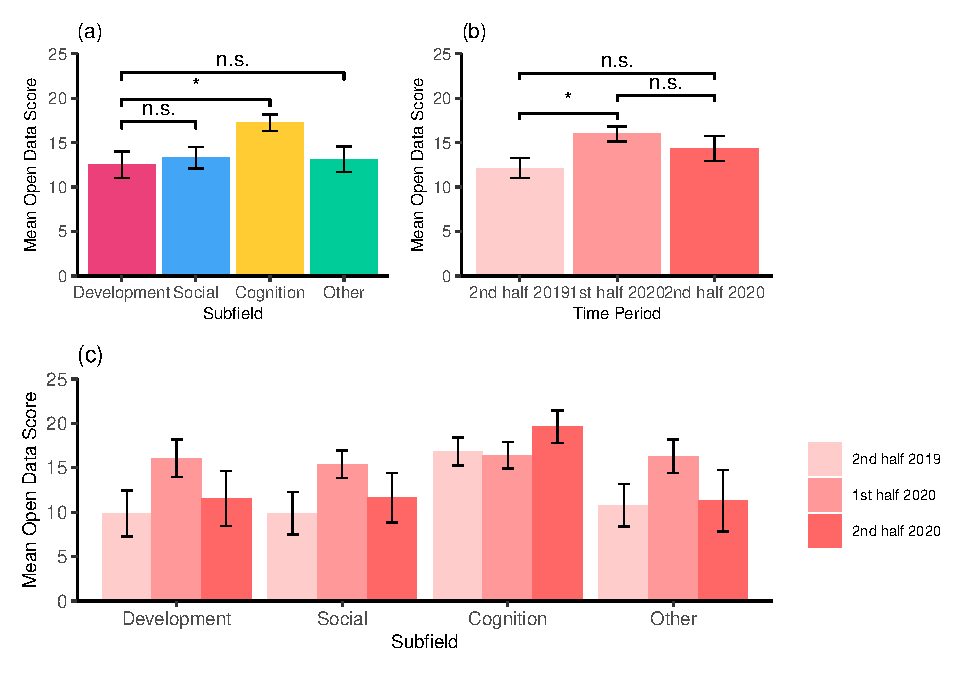
\includegraphics{icd_special_issue_files/figure-latex/1B-d-plots-1.pdf}

\emph{Figure 3}: Mean open data scores for articles published in 2019 and 2020, as a function of subfield and time period.

\begin{table}[tbp]

\begin{center}
\begin{threeparttable}

\caption{\label{tab:1B-m-anova}Between-subjects ANOVA for Open Materials Scores}

\begin{tabular}{lllllll}
\toprule
Effect & \multicolumn{1}{c}{$F$} & \multicolumn{1}{c}{$\mathit{df}_1$} & \multicolumn{1}{c}{$\mathit{df}_2$} & \multicolumn{1}{c}{$\mathit{MSE}$} & \multicolumn{1}{c}{$p$} & \multicolumn{1}{c}{$\hat{\eta}^2_G$}\\
\midrule
Time period & 0.37 & 2 & 181 & 53.87 & .694 & .004\\
Subfield groups & 5.24 & 3 & 181 & 53.87 & .002 & .080\\
Time period $\times$ Subfield groups & 0.48 & 6 & 181 & 53.87 & .822 & .016\\
\bottomrule
\end{tabular}

\end{threeparttable}
\end{center}

\end{table}

\hypertarget{bmaterials-scores-text}{%
\subsection{1BMaterials scores text}\label{bmaterials-scores-text}}

As in Study 1A, for open materials scores in 2019 and 2020, there was a significant main effect of subfield, \(F(3, 181) = 5.24\), \(\mathit{MSE} = 53.87\), \(p = .002\), \(\hat{\eta}^2_G = .080\), however the main effect of time period, \(F(2, 181) = 0.37\), \(\mathit{MSE} = 53.87\), \(p = .694\), \(\hat{\eta}^2_G = .004\), and the interaction between time period and subfield, \(F(6, 181) = 0.48\), \(\mathit{MSE} = 53.87\), \(p = .822\), \(\hat{\eta}^2_G = .016\), were not statistically significant (see Figure 2). Consistent with open data scores, papers published in developmental psychology had significantly lower open materials scores than paper published in cognition, \(t(61.36) = -3.45\), \(p = .001\), however, open materials scores did not differ between developmental and social psychology, \(t(68.36) = -0.84\), \(p = .406\), or between developmental psychology and the other subfield category, \(t(70.45) = -0.62\), \(p = .539\). There were no additional changes in open materials scores across this period between mid-2019 and the end of 2020.

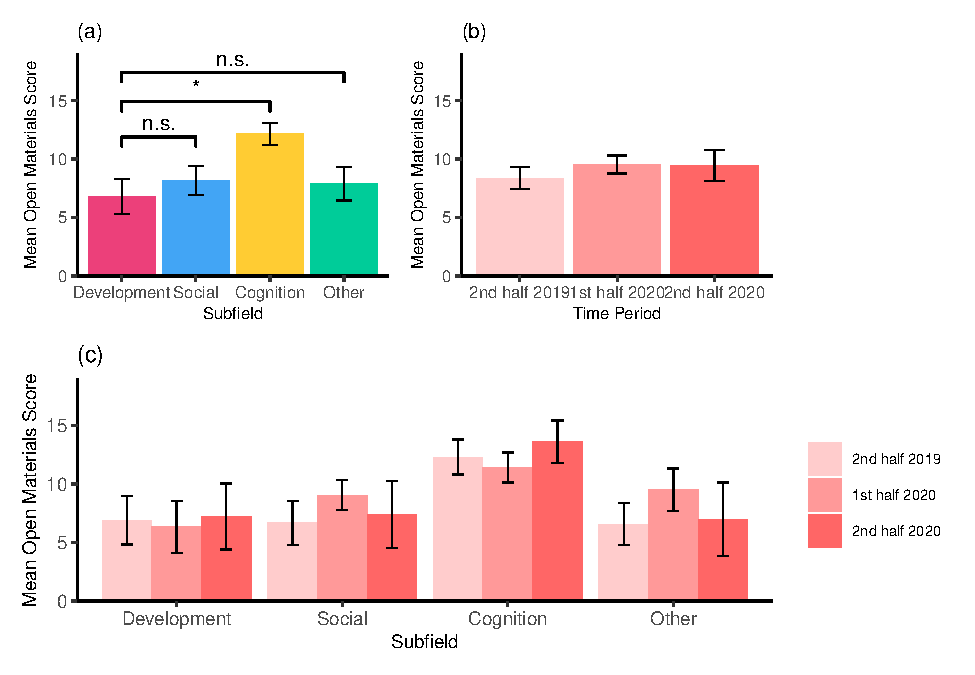
\includegraphics{icd_special_issue_files/figure-latex/1B-m-plots-1.pdf}

\emph{Figure 4}: Mean open materials scores for articles published in 2019 and 2020, as a function of subfield and time period.

\hypertarget{ab-across-time}{%
\section{AB ACROSS time}\label{ab-across-time}}

\hypertarget{ab-datamaterials-text}{%
\section{AB data/materials text}\label{ab-datamaterials-text}}

When looking at open data scores across both time periods, we found that scores increased over time, \(F(1, 507) = 248.98\), \(\mathit{MSE} = 55.28\), \(p < .001\), \(\hat{\eta}^2_G = .329\), and differed as a function of subfield, \(F(3, 507) = 3.74\), \(\mathit{MSE} = 55.28\), \(p = .011\), \(\hat{\eta}^2_G = .022\). However, the interaction between time period and subfield, \(F(3, 507) = 2.28\), \(\mathit{MSE} = 55.28\), \(p = .078\), \(\hat{\eta}^2_G = .013\), was not statistically significant, suggesting that there were no subfield differences in the magnitude of open data scores over time (see Figure Xa). A similar pattern was found for open material scores; scores increased over time \(F(1, 507) = 90.18\), \(\mathit{MSE} = 40.21\), \(p < .001\), \(\hat{\eta}^2_G = .151\), and differed by subfield, \(F(3, 507) = 8.17\), \(\mathit{MSE} = 40.21\), \(p < .001\), \(\hat{\eta}^2_G = .046\), but there was no evidence that the magnitude of improvement over time differed by subfield (see Figure Xb), \(F(3, 507) = 2.07\), \(\mathit{MSE} = 40.21\), \(p = .103\), \(\hat{\eta}^2_G = .012\).

\begin{quote}
t-tests probably not necessary, b/c point was really to see if there was an interaction, also maybe the most appropriate plot is just the interaction one, rather than subfield + time
\end{quote}

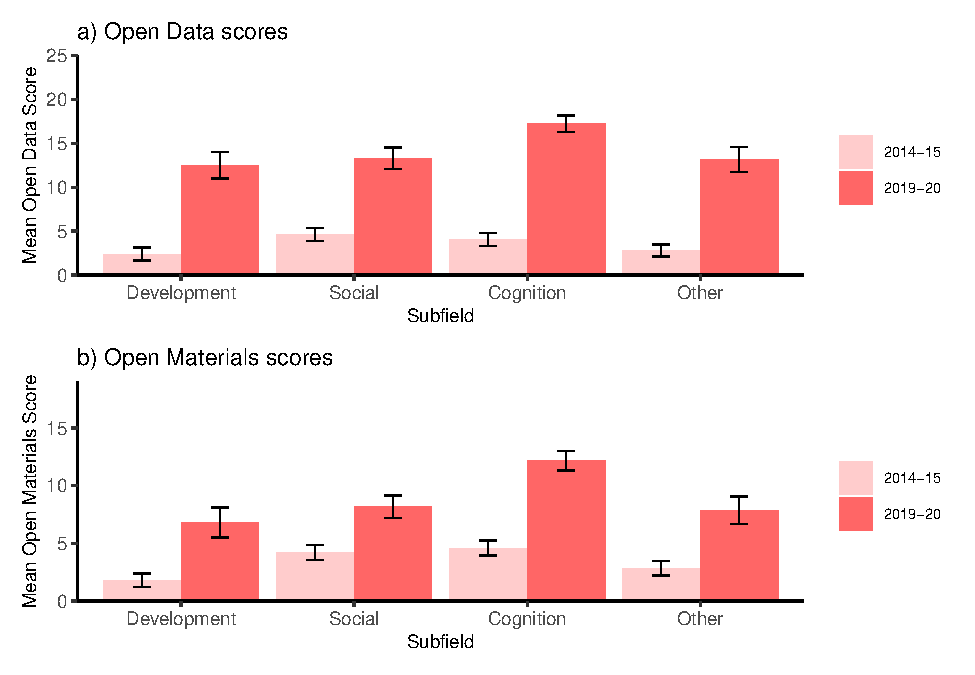
\includegraphics{icd_special_issue_files/figure-latex/AB-m-plot-1.pdf}

\begin{quote}
including just the combo of interaction plots here. Christina- can you remove the code that makes the subfield and time plots from the chunks above and work out how to make this patchwork plot share y axis labels and legends
\end{quote}

\begin{quote}
JENNY UP TO HERE
\end{quote}

\hypertarget{study-1b-exploratory}{%
\section{STUDY 1B EXPLORATORY}\label{study-1b-exploratory}}

\hypertarget{raincloud-plots}{%
\subsection{RAINCLOUD PLOTS}\label{raincloud-plots}}

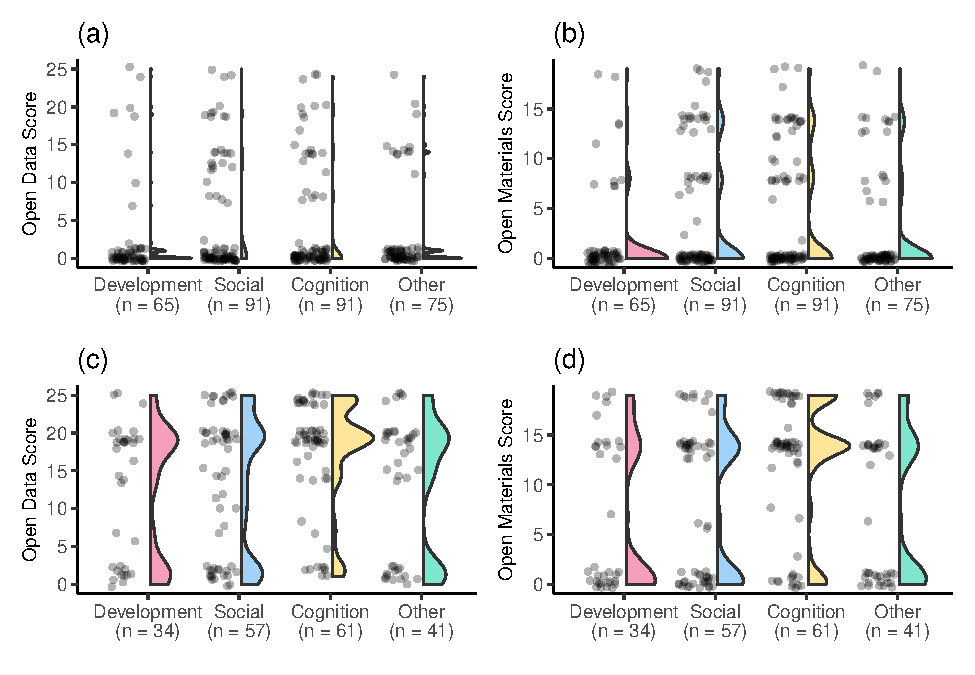
\includegraphics{icd_special_issue_files/figure-latex/1ab-rain-1.pdf}

\hypertarget{open-science-badges}{%
\subsection{OPEN SCIENCE BADGES}\label{open-science-badges}}

\hypertarget{bind-all-statistics-together}{%
\paragraph{Bind all statistics together}\label{bind-all-statistics-together}}

\hypertarget{select-only-relevant-1b-variables}{%
\paragraph{Select only relevant 1B variables}\label{select-only-relevant-1b-variables}}

\hypertarget{summary-tables}{%
\paragraph{Summary tables}\label{summary-tables}}

\hypertarget{combine-1a-and-1b-stats-together}{%
\paragraph{Combine 1A and 1B stats together}\label{combine-1a-and-1b-stats-together}}

\hypertarget{plot-combined-data}{%
\paragraph{Plot combined data}\label{plot-combined-data}}

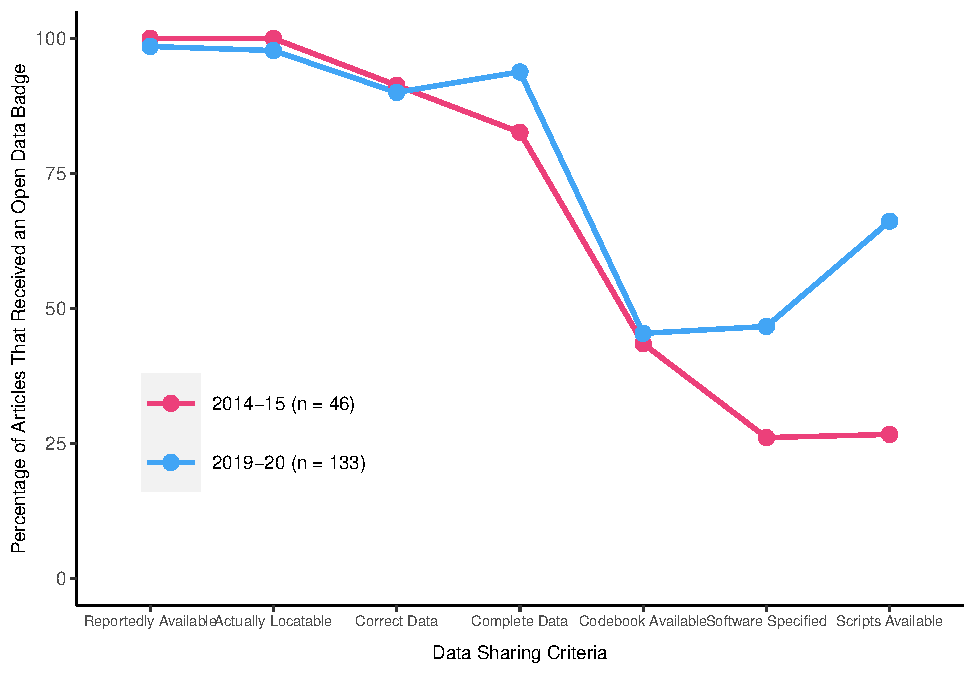
\includegraphics{icd_special_issue_files/figure-latex/combo-plot-1.pdf}

\hypertarget{plot-combined-data-1}{%
\paragraph{Plot combined data}\label{plot-combined-data-1}}

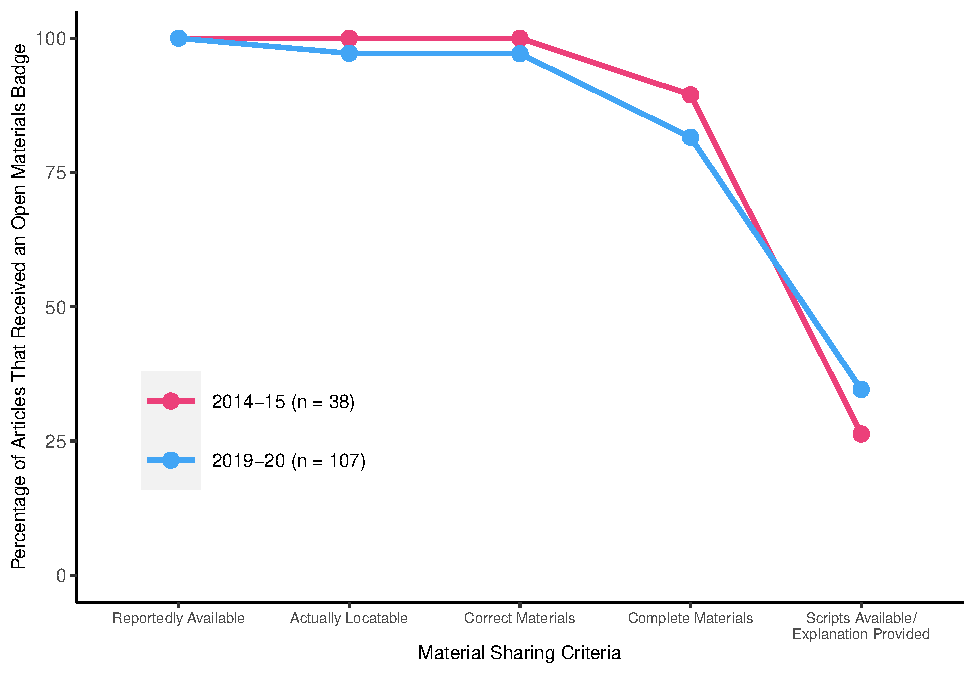
\includegraphics{icd_special_issue_files/figure-latex/combo-m-plot-1.pdf}

\hypertarget{discussion}{%
\section{Discussion}\label{discussion}}

\newpage

\hypertarget{references}{%
\section{References}\label{references}}

\begingroup
\setlength{\parindent}{-0.5in}
\setlength{\leftskip}{0.5in}

\hypertarget{refs}{}
\begin{CSLReferences}{1}{0}
\leavevmode\hypertarget{ref-R-papaja}{}%
Aust, F., \& Barth, M. (2020). \emph{{papaja}: {Create} {APA} manuscripts with {R Markdown}}. Retrieved from \url{https://github.com/crsh/papaja}

\leavevmode\hypertarget{ref-R-Matrix}{}%
Bates, D., \& Maechler, M. (2021). \emph{Matrix: Sparse and dense matrix classes and methods}. Retrieved from \url{https://CRAN.R-project.org/package=Matrix}

\leavevmode\hypertarget{ref-R-lme4}{}%
Bates, D., Mächler, M., Bolker, B., \& Walker, S. (2015). Fitting linear mixed-effects models using {lme4}. \emph{Journal of Statistical Software}, \emph{67}(1), 1--48. \url{https://doi.org/10.18637/jss.v067.i01}

\leavevmode\hypertarget{ref-R-ggeasy}{}%
Carroll, J., Schep, A., \& Sidi, J. (2021). \emph{Ggeasy: Easy access to 'ggplot2' commands}. Retrieved from \url{https://CRAN.R-project.org/package=ggeasy}

\leavevmode\hypertarget{ref-open2015estimating}{}%
Collaboration, O. S. (2015). Estimating the reproducibility of psychological science. \emph{Science}, \emph{349}(6251).

\leavevmode\hypertarget{ref-R-ggsignif}{}%
Constantin, A.-E., \& Patil, I. (2021). {ggsignif}: R package for displaying significance brackets for {'ggplot2'}. \emph{PsyArxiv}. \url{https://doi.org/10.31234/osf.io/7awm6}

\leavevmode\hypertarget{ref-R-janitor}{}%
Firke, S. (2021). \emph{Janitor: Simple tools for examining and cleaning dirty data}. Retrieved from \url{https://CRAN.R-project.org/package=janitor}

\leavevmode\hypertarget{ref-gennetian2020advancing}{}%
Gennetian, L. A., Tamis-LeMonda, C. S., \& Frank, M. C. (2020). Advancing transparency and openness in child development research: opportunities. \emph{Child Development Perspectives}, \emph{14}(1), 3--8.

\leavevmode\hypertarget{ref-R-apa}{}%
Gromer, D. (2020). \emph{Apa: Format outputs of statistical tests according to APA guidelines}. Retrieved from \url{https://CRAN.R-project.org/package=apa}

\leavevmode\hypertarget{ref-R-goodshirt}{}%
Gruer, A. (2021). \emph{Goodshirt: R client for the good place quotes API}.

\leavevmode\hypertarget{ref-hardwicke2018data}{}%
Hardwicke, T. E., Mathur, M. B., MacDonald, K., Nilsonne, G., Banks, G. C., Kidwell, M. C., \ldots{} others. (2018). Data availability, reusability, and analytic reproducibility: Evaluating the impact of a mandatory open data policy at the journal cognition. \emph{Royal Society Open Science}, \emph{5}(8), 180448.

\leavevmode\hypertarget{ref-R-purrr}{}%
Henry, L., \& Wickham, H. (2020). \emph{Purrr: Functional programming tools}. Retrieved from \url{https://CRAN.R-project.org/package=purrr}

\leavevmode\hypertarget{ref-kidwell2016badges}{}%
Kidwell, M. C., Lazarević, L. B., Baranski, E., Hardwicke, T. E., Piechowski, S., Falkenberg, L.-S., \ldots{} others. (2016). Badges to acknowledge open practices: A simple, low-cost, effective method for increasing transparency. \emph{PLoS Biology}, \emph{14}(5), e1002456.

\leavevmode\hypertarget{ref-klein2018practical}{}%
Klein, O., Hardwicke, T. E., Aust, F., Breuer, J., Danielsson, H., Mohr, A. H., \ldots{} others. (2018). A practical guide for transparency in psychological science. \emph{Collabra: Psychology}, \emph{4}(1).

\leavevmode\hypertarget{ref-R-report}{}%
Makowski, D., Ben-Shachar, M. S., Patil, I., \& Lüdecke, D. (2021). Automated results reporting as a practical tool to improve reproducibility and methodological best practices adoption. \emph{CRAN}. Retrieved from \url{https://github.com/easystats/report}

\leavevmode\hypertarget{ref-R-here}{}%
Müller, K. (2020). \emph{Here: A simpler way to find your files}. Retrieved from \url{https://CRAN.R-project.org/package=here}

\leavevmode\hypertarget{ref-R-tibble}{}%
Müller, K., \& Wickham, H. (2021). \emph{Tibble: Simple data frames}. Retrieved from \url{https://CRAN.R-project.org/package=tibble}

\leavevmode\hypertarget{ref-R-patchwork}{}%
Pedersen, T. L. (2020). \emph{Patchwork: The composer of plots}. Retrieved from \url{https://CRAN.R-project.org/package=patchwork}

\leavevmode\hypertarget{ref-R-base}{}%
R Core Team. (2020). \emph{R: A language and environment for statistical computing}. Vienna, Austria: R Foundation for Statistical Computing. Retrieved from \url{https://www.R-project.org/}

\leavevmode\hypertarget{ref-R-afex}{}%
Singmann, H., Bolker, B., Westfall, J., Aust, F., \& Ben-Shachar, M. S. (2021). \emph{Afex: Analysis of factorial experiments}. Retrieved from \url{https://CRAN.R-project.org/package=afex}

\leavevmode\hypertarget{ref-syed2020infant}{}%
Syed, M. (2020). Infant and child development: A journal for open, transparent, and inclusive science from prenatal through emerging adulthood.

\leavevmode\hypertarget{ref-R-gghalves}{}%
Tiedemann, F. (2020). \emph{Gghalves: Compose half-half plots using your favourite geoms}. Retrieved from \url{https://CRAN.R-project.org/package=gghalves}

\leavevmode\hypertarget{ref-R-ggplot2}{}%
Wickham, H. (2016). \emph{ggplot2: Elegant graphics for data analysis}. Springer-Verlag New York. Retrieved from \url{https://ggplot2.tidyverse.org}

\leavevmode\hypertarget{ref-R-stringr}{}%
Wickham, H. (2019). \emph{Stringr: Simple, consistent wrappers for common string operations}. Retrieved from \url{https://CRAN.R-project.org/package=stringr}

\leavevmode\hypertarget{ref-R-forcats}{}%
Wickham, H. (2021a). \emph{Forcats: Tools for working with categorical variables (factors)}. Retrieved from \url{https://CRAN.R-project.org/package=forcats}

\leavevmode\hypertarget{ref-R-tidyr}{}%
Wickham, H. (2021b). \emph{Tidyr: Tidy messy data}. Retrieved from \url{https://CRAN.R-project.org/package=tidyr}

\leavevmode\hypertarget{ref-R-tidyverse}{}%
Wickham, H., Averick, M., Bryan, J., Chang, W., McGowan, L. D., François, R., \ldots{} Yutani, H. (2019). Welcome to the {tidyverse}. \emph{Journal of Open Source Software}, \emph{4}(43), 1686. \url{https://doi.org/10.21105/joss.01686}

\leavevmode\hypertarget{ref-R-dplyr}{}%
Wickham, H., François, R., Henry, L., \& Müller, K. (2021). \emph{Dplyr: A grammar of data manipulation}. Retrieved from \url{https://CRAN.R-project.org/package=dplyr}

\leavevmode\hypertarget{ref-R-readr}{}%
Wickham, H., \& Hester, J. (2021). \emph{Readr: Read rectangular text data}. Retrieved from \url{https://CRAN.R-project.org/package=readr}

\end{CSLReferences}

\endgroup


\end{document}
